\section{Produkt}

\subsection{OTP mit Schweizer Daten implementieren}
Der originale OTP muss mit den Schweizer GTFS-Daten funktionieren, da er als Grundlage für den Algorithmus dient und einen Performancevergleich zwischen den beiden Algorithmen gemacht werden muss. Es gab zwei Probleme, welche dabei behandelt werden mussten.
\newline


Die SBB beschreibt in ihren GTFS-Daten einige Verbindungen mit dem Routentyp 1700 «Miscelaneous». Dieser Typ wird jedoch vom OTP nicht unterstützt da er nicht zugeordnet werden kann. Nach einer Überprüfung der SBB Daten stellte sich heraus, dass der Routentyp 1700 nur für einige Sessellifte sowie Autoverladestationen verwendet wird. Da diese beide nicht in unserem Scope liegen können sie ignoriert werden. Dazu fügten wir dem OTP einen Handler für den Routentyp 1700 hinzu welcher ihn als Auto definiert, da auch das Auto ausserhalb unseres Scpes liegt, jedoch vom OTP unterstützt wird.
\newline


Das zweite Problem war der benötigte Arbeitsspeicher. Für die Grafberechnung mit den SBB GTFS-Daten benötigt der OTP ca. 15 GB Arbeitsspeicher. Die von uns benötigten Rechner konnten diese Speichermenge jedoch nicht zur Verfügung stellen. Deshalb wird für die Berechnung mit den grossen Datensätzen ein Laborcomputer der HTW verwendet. Dieser entspricht mit seinen 32GB Arbeitsspeicher den Anforderungen.


\subsection{Kann OTP ohne .osm file ausgeführt werden?}
Das .osm steht für OpenStreetMap und ist eine Plattform\footnote{\url{https://www.openstreetmap.org/}} die frei nutzbare Daten(sprich Geodaten) zur Verfügung stellt. Wie z.B. Strassen, Wege, Gebäude, Haltestellen usw. OTP kann ohne .osm file ausgeführt werden. Jedoch werden dann keine Fusswege mit einberechnet um zu einer Haltestelle zu gelangen, wie man in Abbildung \ref{fig:ohneosmfile} erkennen kann.
Aber wenn OTP mit dem .osm File ausgeführt wird lässt sich anhand der Informationen einen Gehweg zu der Haltestelle finden (inklusive Laufzeit und Distanz), wie man in Abbildung \ref{fig:mitosmfile} erkennen kann. 

\begin{figure}[htb]
	\centering
	\begin{minipage}{0.45\linewidth}
		\centering
		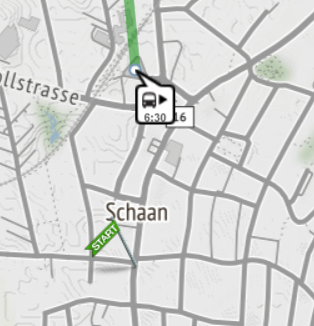
\includegraphics[width=6cm]{img/ohneosmfile.png}
		\caption{ohne .osm File}
		\label{fig:ohneosmfile}
	\end{minipage}
	%\hfill
	\begin{minipage}{0.45\linewidth}
		\centering
		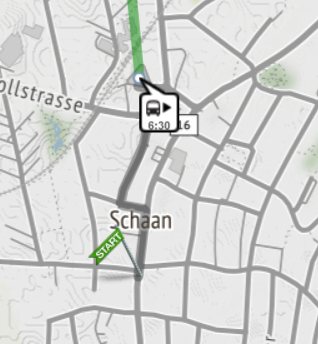
\includegraphics[width=6cm]{img/mitosmfile.png}
		\caption{mit .osm File}
		\label{fig:mitosmfile}
	\end{minipage}
\end{figure}


\subsection{Modellierung der Datenstrukur}
\todocomment{Java container klassen + UML Diagramm}

\subsection{Automatische generierte Klassendiagramme}
Klassendiagramme können sehr behilflich sein bei der Entwicklung. Sie geben einen Überblick welche Klassen miteinander agieren.
Der Opentripplaner besteht aus unzähligen verschiedenen Klassen. Um eine bessere Übersicht zu erhalten erzeugten wir mit dem Programm objectaid\footnote{\url{http://www.objectaid.com/home}} (ein Plugin für Eclipse) fast vollautomatisch Klassendiagramme. 

%beispielbild eines Klassendiagramms mit objectaid ?

\subsection{Dummy-GTFS Daten erstellen}
Wir haben selbst GTFS-Daten erstellt, weil ein komplettes Schweizer-GTFS schon ein paar Stunden braucht um die Daten einzulesen. So brauchen wir nicht bei jedem Ausführen des Programms jedes mal ein paar Stunden zu warten, was uns bei der Entwicklung viel Zeit erspart. Dadurch das wir dieses GTFS-Daten selber erstellt haben, wissen wir nun was genau vorhanden ist und können dadurch nachvollziehen ob z.B. Die GTFS-Daten richtig eingelesen wurden und daraus auch weitere Methoden auf ihre Richtigkeit Überprüfen kann.\newline

Das Dummy-GTFS wurde anhand der bestehenden Schweizer-GTFS Daten erstellt. Im Schweizer-GTFS sind auch die Daten des öffentlichen Verkehrs von Liechtenstein enthalten. Wir haben uns entschieden nur ein Teil der Liechtensteinischen Busverbindungen zu übernehmen und selber zu erstellen um den Inhalt der Schweizer-GTFS Daten beizubehalten.

\begin{figure}[h]
	\centering
	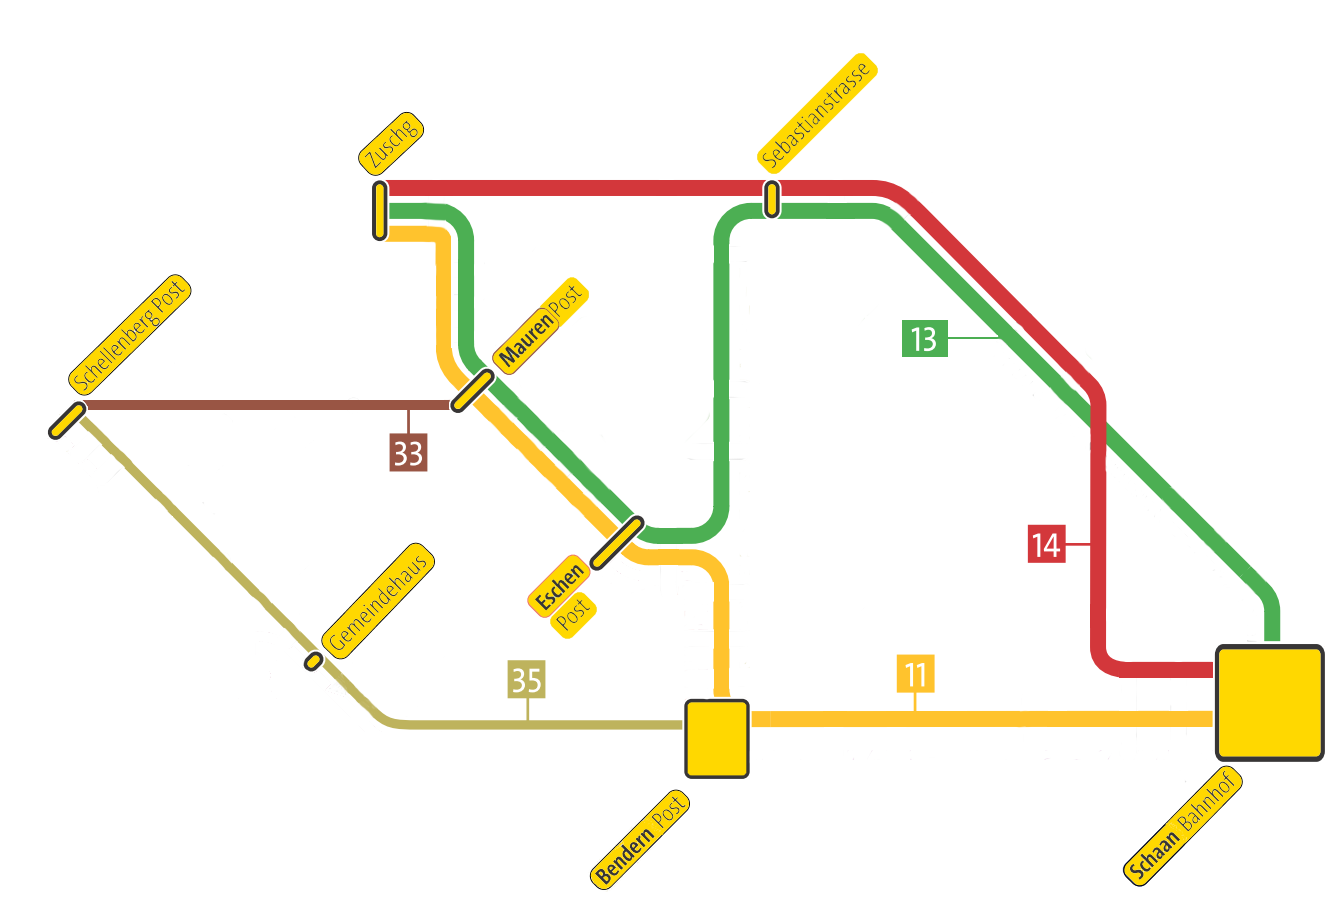
\includegraphics[width=12cm]{img/LiniennetzDummyGTFS.png}
	\caption{Dieses Bild gibt eine Übersicht welche Haltestellen und Routen im Dummy-GTFS vorhanden ist.}
	\label{fig:DummyGTFS-uebersicht}
\end{figure}

\subsection{Mocking}
Das Programm kann grob in drei Abschnitte aufgeteilt werden. Das erstellen des Zeitplans aus den GTFS-Daten, den Wegfindungsalgorithmus und einen Converter welcher das Resultat in die von der Webseite verlangte Form bringt. Damit diese drei Abschnitte separat behandelt werden konnten und das Programm dennoch jederzeit überprüft werden konnte entschieden wir uns ein Mockup für die Abschnitte durchzuführen.

\subsubsection{CSAMock}
Das Mocking des CSA bekommt ein Zeitplan-Objekt als Eingabe und speichert dieses zur Kontrolle in einem JSON-File. Danach wird manuell ein Journey erstellt welches eine Reise von «Heerbrugg, Dornacherhof» nach «Heerbrugg, Bahnhof» repräsentiert. Diese Verbindung wurde gewählt, da es eine einfache Busfahrt ohne Zwischenstops ist. Dieser Journey wird dann als Antwort zurückgegeben.

\subsubsection{TimeTableBuilderMock}
Das Mocking des TimeTableBuilders erstellt manuell einen Zeitplan mit zwei Haltestellen und einer Busverbindung. Dieser wird anschliessend als Response zurückzugeben.

\subsubsection{JourneyToTripPlanConverterMock}
Der als Parameter bekommene Journey wird zur Überprüfung in ein JSON-File gespeichert. Anschliessend wird manuell eine Webseitenantwort aufgebaut. Anfangs wurde eine Reise ohne Zwischenstops, Umsteigen und Fusswege zurückgegeben. Doch in folgenden Schritten wurde das Mocking erweitert um die zuvor erwähnten, komplexeren Fälle zu behandeln.

\subsection{TimeTableBuilder}
Die Aufgabe des TimeTableBuilder ist es Daten aus dem GTFS zu lesen und anschliessend eine Datenstruktur daraus zu erzeugen die der Connection Scan Algorithm benötigt. Zum einlesen der GTFS-Daten wird die Onebusaway Library verwendet. Diese erzeugt anhand der Daten Objekte.Die Objektdaten von der Onebusaway Library sind in Listen abrufbar.
z.B. Entspricht im GTFS Stop.txt ein Zeileneintrag einem Stop Objekt. Durch diese Library ist es einfacher Daten aus dem GTFS abzufragen. z.B. von einem Stop kann man gezielt nach dem Namen fragen\texttt{stop.getName()}.\newline  

Da ein Stop aus der Library gleich bei uns heissen würde. Führt dies zu einem Namenskonflikt mit der Klasse Stop für den CSA und Stop von der onebusaway Library. Um dieses Problem zu lösen benannten wir die Klassen, die wir benötigen werden für den CSA um. Indem wir die Klassen mit der CSA Endung erweiterten z.B. Stop in StopCSA.\newline

Durch diese Library lässt es sich nun relativ einfach die Daten aus dem GTFS lesen und anschliessend mit den gewünschten Daten die benötigten Objekte erstellen.Dafür wir die Funktion \texttt{.loadFromGtfs()} ausgeführt.  Stop, Footpath und Trips lassen sich relativ leicht erstellen weil die GTFS-Daten hierbei schon in sehr ähnlich Form aufgebaut sind. Jedoch ist es bei der Connection etwas schwieriger, da die Daten nicht in dieser Art direkt vorhanden sind. Die Connections müssen beim der Stop\_times.txt immer zwei hintereinanderfolgende Einträge(Objekte) vergleichen um zu Erkennen das es sich um eine Connection handelt. Eine Connection wird erkannt wenn sie auf den selben Trip stattfinden und die stop\_sequence Zahl muss grösser sein als der vorhergehende Eintrag. Wenn dieser Fall nur Zutrifft wurde eine Connection erkannt. Bevor jetzt aber das Connection Objekt einfach erzeugt werden kann müssen noch die richtigen Referenzen gefunden werden. Den die Stops und Trips wurden zuvor schon erzeugt. Den eine Connection muss wissen auf welchem Trip sie ist und welche Departure- und ArrivalStops sie enthält. Nachdem also eine Connection gefunden wurde wird er richtige Trip in der bestehenden Liste gesucht, anhand der TripId kann der Trip aus der Liste gefunden werden. Das selbe geschieht auch mit den Departure- und ArrivalStops. Wenn alle Informationen gefunden wurden wird das Connection Objekt erzeugt und in das TreeSet(sortiere Liste) übergeben. Durch die \texttt{.compareTo()} Funktion der Connection lässt sie sich an der richtigen Stelle im TreeSet einfügen. Somit bekommen wir alle Connections sortiert nach der Departuretime. Am Ende der Funtion wird ein Java-SerializedObjectFile vom TimeTable erstellt. Somit wird das gewünschte Format zwischengespeichert. Das erstellen dieser Datei benötigt nur 1-2 Minuten und die Datei ist 367MB gross.\newline

Die Funktion \texttt{.loadFromGtfs()} benötigt etwa 60h um das Schweizer GTFS einzulesen. Aber durch Optimierung konnte die Zeit veringert werden auf 22h. Indem wir die nicht mehr einfach wie vorher ständig nach dem Trip wieder suchen wenn eine Connection gefunden wurde. Durch zwischenspeichern der Referenz des vorhergehenden Trips kann dieser wiederverwendet werden, wenn die TripId der Einträge übereinstimmen. Somit muss nur ein Trip in der Liste gesucht werden wenn diese TripId nicht übereinstimmen. Zudem kann durch zwischenspeichern der Referenz auf den vorhergehenden Stop eine Suche in der Liste vermieden werden. Da ein Trip und Stop nur einmal vorkommt in der Liste, kann beim durchlaufen mit einer Suchschleife die suche nach dem Trip vorzeitig abgebrochen werden, was verhindert das unnötig weiter nachdem Trip/Stop gesucht wird.  

Die Funktion \texttt{.loadFromSerializedObjectFile()} kann verwendet werden um zwischengespeicherte TimeTables einzulesen. Das SerializedObjectFile das zuvor aus dem Schweizer GTFS erstellt wurde lässt sich innerhalb von 151s einlesen.


\subsection{JourneyToTripPlanConverter}
Der JourneyToTripPlanConverter bildet einen von der Webseite benötigten TripPlan aus den vom CSA generierten Journeys. Aus dem Mocking sind die benötigten Parameter schon bekannt so dass die Generierung nun nur noch automatisiert werden muss. Dabei gab es jedoch mehrere Punkte welche speziell beachtet werden mussten.
\begin{enumerate}
	\item Ein Journey besitzt nur eine Dauer für den kompletten Weg. Der TripPlan jedoch speichert sich separate Werte für Fahrzeit, Laufzeit und Wartezeit. Die Fahrzeit und die Laufzeit können dabei einfach aus den Start- und Stop-Zeiten der Legs oder Footpaths übernommen werden. Bei der Wartezeit beseht jedoch das Problem das sie den Zeitunterschied zwischen zwei Abschnitten repräsentiert. Dies bedeutet, dass in der Schleife die beiden zu vergleichenden Zeiten nicht gleichzeitig vorhanden sind. Dieses Problem wird umgangen indem die Endzeit des Itinerarys nach jedem berechneten Leg angepasst wird. Somit stimmt dieser Wert immer mit der Endzeit des Legs des vorhergehenden Schleifendurchgangs überein. 
	\item Jedes Leg im TripPlan benötigt ein LegGeometry-Object. Dies wird benötigt damit die Webseite eine Linie entlang des Fahrtweges anzeigen kann. Dies wird mithilfe der GeometryUtils-Bibliothek und den Start- und Endkoordianten eine Gerade erstellt. Diese 
	\item Im TripPlan wird ein Fussweg mithilfe von verschiedenen WalkSteps definiert. Diese benötigen jedoch eine Variable AbsoluteDirection welche 8 Himmelsrichtungen repräsentiert. Diese musste in einer komplexen Winkelberechnung aus den Koordinaten berechnet werden. Danach wird der Winkel auf 45 Grad Abschnitte gerundet und den jeweiligen Himmelsrichtungen zugeordnet.
	\item Der CSA stellt sowohl Fusswege als auch Umsteigeprozesse als Footpaths dar. Umsteigeprozesse werden aber vom TripPlan nicht dargestellt, ausser das sie in die Zeitberechnung miteinfliessen müssen. Daher müssen die Fusswege und Umsteigeprozesse unterschieden werden. Nachdem ein Leg generiert wurde, jedoch noch bevor es der Liste von Legs hinzugefügt wurde, wird überprüft, ob die Start- und Zielkoordianten gleich sind. Ist dies der Fall so handelt es sich um einen Umsteigeprozess und das berechnete Leg wird der Liste nicht hinzugefügt. Die berechneten Zeiten werden jedoch trotzdem für das nächste Leg verwendet.
\end{enumerate}

\subsection{ConnectionScanAlgorithm}
Von den beiden CSA-Versionen kümmerten wir uns zuerst um den Earliest Arrival Scan Algorithmus, da dieser weniger Komplex ist und als Grundlage für den Profile Connection Scan Algorithmus dient.
\subsubsection{EAS}
Am Anfang werden für alle Stops und Trips Handler angelegt. Handler sind Hilfskonstruktionen welche alle informationen der Stops und Trips beinhalten, welche im verlauf der Berechnung geändert werden müssen wie zum Beispiel die EinstiegsConnection für die Trips. Das ist nötig, da wir mit einem persistenten TimeTable-Objekt arbeiten welches für die nächsten Anfragen nicht verändert werden darf.
\newline


Danach werden die Zeitvariabeln vorbereitet. Das Jahr, der Monat und der Tag müssen aus dem Request übernommen werden, da die Zeitangaben des Zeitplans nur auf die Uhrzeit und nicht auf das Datum beziehen. Dazu werden die Datumswerte in Variablen gespeichert.  Nun wird im Stop-Handler des Startstops die Startzeit des Requests eingetragen. Für alle anderen Stop-Handler wird die zeit auf den 31.12.20000 gesetzt. Diese Zeit simuliert eine Unendlich grosse Zahl welche trotzdem noch mit den Calendar-Methoden verglichen werden kann.
\newline


Dann werden alle aufsteigend nach Abfahrtszeit sortierten Connections durchlaufen. Für jede Connection wird überprüft, ob die im Stop-Handler des Startstops der Connection gespeicherte Zeit vor der abfahrtszeit der Connection ist, oder ob im zur Connection passenden Trip-Handler das Trip-Bit gesetzt ist. Das Trip-Bit ist am Start auf «false» gesetzt. Sobald eine Connection gefunden wird welche eine der zwei vorherigen Bedingungen erfüllt so wird es für den zur Connection passenden Trip auf True gesetzt. Damit werden sich erreichbare Verkehrsmittel gemerkt, so dass weitere Connections im gleichen ÖV auch als erreichbar markiert sind. Die zweite Bedingung prüft ob der Startstop der Connection schon erreicht wurde. Anfangs ist nur die Zeit im Stop-Handler des Startstops gesetzt. Alle anderen Zeiten sind auf Unendlich gesetzt. Somit werden nur Connections behandelt welche vom Startstop ausgehen und später abfahren als die im Request definierte Startzeit. Sobald so eine Connection gefunden wurde wird die Ankunftszeit in den Stop-Handler des Ankunftsstops der Connection geschrieben. Somit ist nun auch dieser als erreichbar markiert und wird bei weiteren Durchläufen beachtet. Zusätzlich wird jedesmal wenn eine Connection gefunden wurde ein JourneyPointer im Stophandler des Ankunftsstops der Connection gespeichert, um den Journey später rekonstruieren zu können.
\newline


Das Breakkriterium für die Schleife ist wenn die Abfahrtszeit der Connection später ist als die im Stop-Handler des Zielstops gespeicherte Zeit. Diese Zeit ist auf Unendlich gesetzt und wird erst neu gesetzt wenn ein Journey zum Zielpunkt gefunden wurde. Da die Connections aufsteigend nach Abfahrtszeit durchlaufen werden ist dies auch automatisch die am Frühesten ankommende Reise. 
\newline


Nun wird vom Zielstop aus der Journey rekonstruiert. Im JourneyPointer des Zielstops steht der zuvor erreichte Stop. Nun wird der JourneyPointer dieses neuen Stops untersucht. Dies wird so lange wiederholt bis der Startstop erreicht ist. Nun werden die gefundenen Stops in umgekehrter Reihenfolge in den Journey eingetragen und der Journey wird zurückgegeben.
\subsubsection{PCS}
Der Profile Connection Scan Algorithmus erstellt am Anfang auch Stop- und Triphandler sowie die im EAS erwähnten Zeitvariabeln. Danach werden die Verbindungen in einer Schleife durchlaufen. Im Gegensatz zum EAS werden sie jedoch absteigend nach Abfahrtszeit durchlaufen. Damit jedoch nur ein Zeitfenster der Verbindungen um die gesuchte Zeit herum behandelt werden muss wird vor der Schleife ein EAS durchgeführt, welcher nur die früheste Ankunftszeit zurückliefert. Dieser Zeit werden dann zwei Stunden hinzugerechnet und sie wird als Einstugspunkt für die Schleife benutzt. 
\newline


Nun werden drei Zeitvariablen gesetzt. Die erste zeigt wann und ob man ans Ziel kommt, wenn man aus dem ÖV aussteigt. Dies ist nur der Fall, wenn der Ankunftsort der Connection dem Zielort entspricht. In diesem Fall wird die Ankunftszeit der Connection in der Zeitvariable gespeichert. Ist dies nicht der fall so wird sie auf Unendlich gesetzt.
\newline


Die zweite Zeitvariable zeigt wann und ob man ans Ziel kommt, wenn man im ÖV sitzen bleibt. Dabei wird die TripZeit in der Zeitvariablen gespeichert. Ist diese ungleich unendlich so ist das Zeil mit weiterfahren erreichbar.
\newline


Die dritte Zeitvariable zeigt wann und ob man ans Ziel kommt, wenn man in ein anderes ÖV umsteigt. Dazu werden alle TimeTupels im Zielstop aufsteigend durchlaufen bis eine TimeTupel gefunden wurde, welches später abfährt als die Ankunftszeit der Connection plus die Umsteigezeit. Da jeder Stop ein default TimeTupel mit der Zeit Unendlich hat wird immer eine Möglichkeit gefunden. 
Danach werden die drei Zeitvariablen verglichen und der früheste wird behalten. Dies ist nun die schnellste Zeit in welcher man von dieser Connection aus das Ziel erreichen kann. Nun wird von der Abfahrtszeit der Connection die Umsteigzeit abgezogen und es wird mit diesen beiden Zeiten ein neues TimeTupel erstellt. Nun wird überprüft ob die Ankunftszeit nicht unendlich ist und somit der Zielort erreichbar ist. Wenn dies der Fall ist so wird das Tupel zusammen mit einen JourneyPointer in den Stop-Handler geschrieben, für den Trip wird eine TripZeit festgelegt und falls für diesen Trip noch keine ExitConnection festgelegt ist wird die aktuelle Connection eingetragen. Dies wird so lange wiederholt bis die Abfahrtszeit der Connection vor der im Request spezifizierten Startzeit ist.
\newline


Nun werden die Journeys vom Startstop aus rekonstruiert. Es wird ein Journey für jedes im Startstop gespeichertes TimeTupel generiert. Dabei wird erste JourneyPointer im Journey eingetragen. Dann werden die im Endstop des Journeys gespeicherten TimeTupels überprüft. Hierbei wird nur das erste Tupel und nicht alle verwendet. Diese Entscheidung wurde aus performance Gründen getroffen, da die Anzahl an schritten ansonsten Exponenziell ansteigen würde. Dies wird so lange wiederholt bis der Zeilstop erreicht ist. 
\newline


Der Vorgang benötigt jedoch noch einen Zusatz, da der Algorithmus auch Reisen findet, welche Kreise fahren und den selben Ort mehrfach anfahren. Um dies zu verhindern wird eine Liste mit allen schon angefahrenen Stops geführt. Für jeden neuen JourneyPointer wird geprüft ob der Ankuftsstop schon in der Liste vorhanden ist. Ist dies der Fall so wird ein Bit auf TRUE gesetzt. Am ende werden nur Journey der Rückgabe hinzugefügt bei welchen kein Stop mehrfach angefahren wurde.

\subsection{Performance-Test}
Um den Performance-Test durchzuführen wird ein JUNIT-Test mit der JUNIT-Benchmark erweiterung genutzt. Dieser führt mehrere Requests durch. Ein Reqeust ohne Umsteigen. Einer mit einmal Umsteigen und einer mit zweimal umsteigen.
\newline


Die Tests schlugen jedoch bei dem CSA ohne die QuadTree-Optimierung fehl, da die Anfrage mit den kompletten Schweizer-Daten länger als 24 Stunden dauerte.




